\documentclass[11pt,letterpaper]{article}
\usepackage[margin=2.5cm]{geometry}
\usepackage[utf8]{inputenc}
\usepackage[T1]{fontenc}
\usepackage{lmodern}
\usepackage{amsmath,amssymb,amsthm,mathtools,bm}
\usepackage{enumitem}
\usepackage{booktabs}
\usepackage{tikz}
\usetikzlibrary{arrows.meta,patterns,positioning,calc}
\usepackage{pgfplots}
\pgfplotsset{compat=1.16}
\usepackage{titlesec}
\usepackage[hidelinks]{hyperref}

\setlength{\parindent}{0pt}
\setlength{\parskip}{0.5em}
\titleformat{\section}{\large\bfseries}{\thesection.}{0.6em}{}
\titleformat{\subsection}{\normalsize\bfseries}{\thesubsection.}{0.6em}{}

\theoremstyle{definition}
\newtheorem{definition}{Definition}[section]
\newtheorem{example}{Example}[section]
\newtheorem{exercise}{Exercise}[section]
\newtheorem{theorem}{Theorem}[section]
\newtheorem{remark}{Remark}[section]

\newcommand{\R}{\mathbb{R}}
\newcommand{\N}{\mathbb{N}}
\newcommand{\Z}{\mathbb{Z}}
\newcommand{\U}{\mathcal{U}}
\newcommand{\E}{\mathbb{E}}
\newcommand{\Var}{\operatorname{Var}}
\newcommand{\Cov}{\operatorname{Cov}}
\newcommand{\Normal}{\mathcal{N}}
\newcommand{\dd}{\,\mathrm{d}}
\newcommand{\T}{^{\top}}
\renewcommand{\P}{P}
\newcommand{\set}[1]{\left\{#1\right\}}
\newcommand{\given}{\mid}
\newcommand{\note}[1]{\textit{#1}}

\title{Lecture 10: Hierarchical Models}
\author{}\date{}

\usetikzlibrary{fit}
\tikzset{
  rv/.style={circle, draw, minimum size=9mm, inner sep=0pt},
  fixed/.style={inner sep=1pt},
  edge/.style={-{Stealth[length=2mm]}},
  plate/.style={draw, rectangle, inner sep=6pt},
  plabel/.style={font=\footnotesize, inner sep=1pt}
}

\begin{document}
\maketitle

%=====================================================
\section{Grouped data}
Consider data involving several related groups. Each observation $y_{ij}$ belongs to a group $j = 1, \dots, J$, and $i = 1, \dots, n_j$ indexes units within the group. Each group has a total of $n_j$ observations.

\begin{example}
\leavevmode
\begin{enumerate}[label=\arabic*.)]
  \item Survival rates at different hospitals.
  \item Waiting times at different caf\'es.
  \item Air pollution measured from different stations.
\end{enumerate}
\end{example}

%=====================================================
\section{Complete, no and partial pooling}
\textbf{Complete pooling:} if groups were identical, then we'd need just one parameter $\theta$ shared by all groups.

\textbf{No pooling:} groups are completely different and they can be described only through parameters $\theta_j$ that depend only on $y_{ij}$.

\textbf{Partial pooling:} there is a hyperparameter that describes the population of groups. For these cases hierarchical models are appropriate.

Assuming that the prior on the hyperparameters $\phi$ is fixed,
\begin{align*}
p(\phi, \theta, y) &= p(\theta, y \given \phi)\,p(\phi), \\
p(\theta, y \given \phi) &= p(y \given \theta, \phi)\,p(\theta \given \phi),
\end{align*}
so
\[
p(\phi, \theta, y) = p(\phi)\,p(\theta \given \phi)\,p(y \given \theta, \phi),
\]
and since the data depend on $\phi$ only through $\theta$, $p(y \given \theta, \phi) = p(y \given \theta)$:
\[
\phi \longrightarrow \theta \longrightarrow y.
\]
$\theta$ already contains the information about $\phi$.

If $y_j$ is a dataset with units $y_{ij}$, $i = 1, \dots, n_j$, one could fit a model
\[
p(\theta_j \given y_j)
\]
for each group. That could give poor results if $y_j$ is small. We could instead pool all the data and fit a model $p(\theta \given y)$ for all the data $y$.

%=====================================================
\section{A hierarchical model and its plate diagram}
For example, with $\phi = (\mu, \sigma)$:
\begin{center}
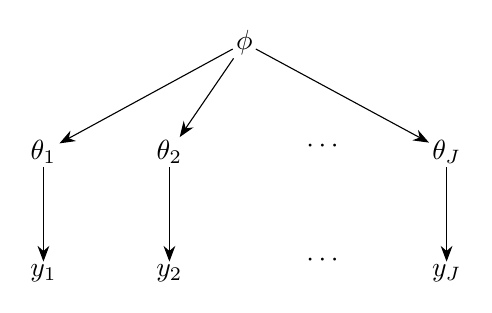
\begin{tikzpicture}[node distance=12mm and 14mm]
  \node[fixed] (phi) {$\phi$};
  \node[fixed, below left=10mm and 22mm of phi] (t1) {$\theta_1$};
  \node[fixed, below left=10mm and 6mm of phi] (t2) {$\theta_2$};
  \node[fixed, below right=10mm and 6mm of phi] (td) {$\cdots$};
  \node[fixed, below right=10mm and 22mm of phi] (tJ) {$\theta_J$};
  \node[fixed, below=of t1] (y1) {$y_1$};
  \node[fixed, below=of t2] (y2) {$y_2$};
  \node[fixed, below=of td] (yd) {$\cdots$};
  \node[fixed, below=of tJ] (yJ) {$y_J$};
  \foreach \t in {t1,t2,tJ} \draw[edge] (phi) -- (\t);
  \draw[edge] (t1) -- (y1); \draw[edge] (t2) -- (y2); \draw[edge] (tJ) -- (yJ);
\end{tikzpicture}
\end{center}

The same model drawn as a plate diagram, in general and with $\phi = (\mu, \sigma^2)$:
\begin{center}
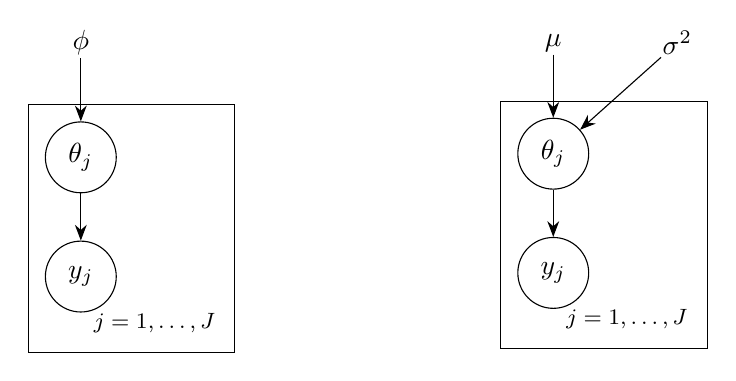
\begin{tikzpicture}
  \begin{scope}
    \node[fixed] (phi) {$\phi$};
    \node[rv, below=8mm of phi] (th) {$\theta_j$};
    \node[rv, below=6mm of th] (y) {$y_j$};
    \draw[edge] (phi) -- (th); \draw[edge] (th) -- (y);
    \node[plabel, below right=1mm and -2mm of y] (l1) {$j = 1, \dots, J$};
    \node[plate, fit=(th)(y)(l1)] {};
  \end{scope}
  \begin{scope}[xshift=60mm]
    \node[fixed] (mu) {$\mu$};
    \node[fixed, right=12mm of mu] (s2) {$\sigma^2$};
    \node[rv, below=8mm of mu] (th2) {$\theta_j$};
    \node[rv, below=6mm of th2] (y2) {$y_j$};
    \draw[edge] (mu) -- (th2); \draw[edge] (s2) -- (th2); \draw[edge] (th2) -- (y2);
    \node[plabel, below right=1mm and -2mm of y2] (l2) {$j = 1, \dots, J$};
    \node[plate, fit=(th2)(y2)(l2)] {};
  \end{scope}
\end{tikzpicture}
\end{center}

The joint distribution factorizes as
\begin{align*}
p(\phi, \theta, y) &= p(\phi)\,p(\theta \given \phi)\,p(y \given \theta) \\
&= p(\phi)\prod_{j=1}^{J}p(\theta_j \given \phi)\,p(y_j \given \theta_j).
\end{align*}
We want to infer the parameters given the data. This is
\[
p(\phi, \theta \given y) = \frac{p(\phi, \theta, y)}{p(y)},
\]
with the generative model
\begin{align*}
\mu &\sim p(\mu), \\
\sigma &\sim p(\sigma), \\
\theta_j \given \mu, \sigma &\sim p(\theta_j \given \mu, \sigma), \qquad j = 1, \dots, J, \\
y_j \given \theta_j &\sim p(y_j \given \theta_j), \qquad j = 1, \dots, J.
\end{align*}

%=====================================================
\section{Another example: varying intercepts and slopes}
\begin{center}
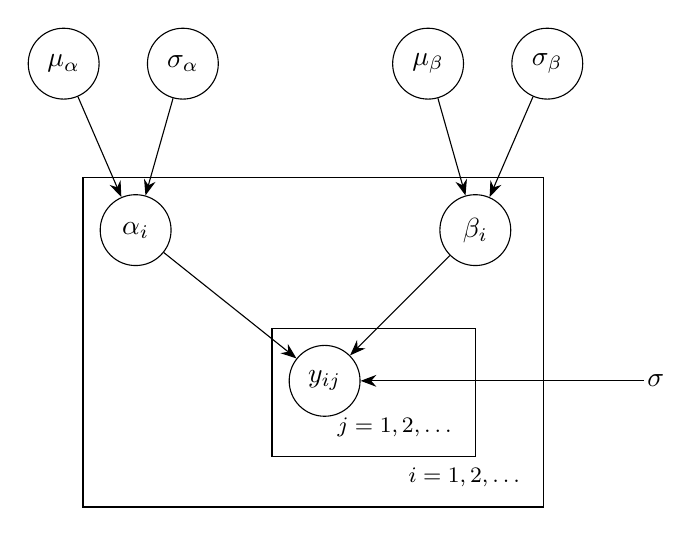
\begin{tikzpicture}
  \node[rv] (ma) {$\mu_\alpha$};
  \node[rv, right=6mm of ma] (sa) {$\sigma_\alpha$};
  \node[rv, right=22mm of sa] (mb) {$\mu_\beta$};
  \node[rv, right=6mm of mb] (sb) {$\sigma_\beta$};
  \node[rv, below=12mm of sa, xshift=-6mm] (a) {$\alpha_i$};
  \node[rv, below=12mm of mb, xshift=6mm] (b) {$\beta_i$};
  \node[rv, below=10mm of a, xshift=24mm] (y) {$y_{ij}$};
  \node[fixed, right=36mm of y] (s) {$\sigma$};
  \draw[edge] (ma) -- (a); \draw[edge] (sa) -- (a);
  \draw[edge] (mb) -- (b); \draw[edge] (sb) -- (b);
  \draw[edge] (a) -- (y); \draw[edge] (b) -- (y); \draw[edge] (s) -- (y);
  \node[plabel, below right=1mm and -2mm of y] (lj) {$j = 1, 2, \dots$};
  \node[plate, fit=(y)(lj)] (pj) {};
  \node[plabel, below right=1mm and 4mm of pj.south] (li) {$i = 1, 2, \dots$};
  \node[plate, fit=(a)(b)(pj)(li)] {};
\end{tikzpicture}
\end{center}

\begin{align*}
p(\mu_\alpha, \sigma_\alpha, \mu_\beta, \sigma_\beta, \alpha, \beta, \sigma, y)
&= p(\mu_\alpha)\,p(\sigma_\alpha)\,p(\mu_\beta)\,p(\sigma_\beta)\,p(\sigma) \\
&\quad\times \prod_{i=1}^{I}\left[p(\alpha_i \given \mu_\alpha, \sigma_\alpha)\,p(\beta_i \given \mu_\beta, \sigma_\beta)\prod_{j=1}^{J}p(y_{ij} \given \alpha_i, \beta_i, \sigma)\right],
\end{align*}
with
\begin{align*}
\mu_\alpha &\sim p(\mu_\alpha), \qquad \sigma_\alpha \sim p(\sigma_\alpha), \\
\mu_\beta &\sim p(\mu_\beta), \qquad \sigma_\beta \sim p(\sigma_\beta), \\
\alpha_i \given \mu_\alpha, \sigma_\alpha &\sim p(\alpha_i \given \mu_\alpha, \sigma_\alpha), \qquad i = 1, \dots, I, \\
\beta_i \given \mu_\beta, \sigma_\beta &\sim p(\beta_i \given \mu_\beta, \sigma_\beta), \qquad i = 1, \dots, I, \\
y_{ij} \given \alpha_i, \beta_i, \sigma &\sim p(y_{ij} \given \alpha_i, \beta_i, \sigma), \qquad i = 1, \dots, I,\ j = 1, \dots, J.
\end{align*}

%=====================================================
\section{Example: eight schools}
Run a coaching program to prepare students for the SAT verbal test. Some students get coached and others don't. Everyone took the test. We compare the two groups' scores, given each school's estimated effect $y_j$.

$y_j$ is a number for each school ($j$ labels schools):
\[
y_j = \text{average score (coached)} - \text{average score (uncoached)},
\]
and $\sigma_j$ is its standard error. The model for the observed effect is
\[
y_j = \theta_j + \varepsilon_j, \qquad \varepsilon_j \sim \Normal(0, \sigma_j^2).
\]

\begin{center}
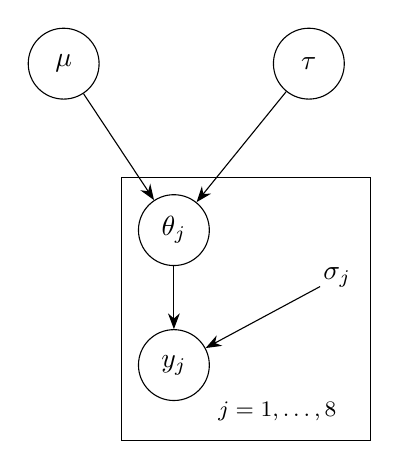
\begin{tikzpicture}
  \node[rv] (mu) {$\mu$};
  \node[rv, right=22mm of mu] (tau) {$\tau$};
  \node[rv, below=12mm of mu, xshift=14mm] (th) {$\theta_j$};
  \node[rv, below=8mm of th] (y) {$y_j$};
  \node[fixed, right=14mm of th, yshift=-6mm] (sj) {$\sigma_j$};
  \draw[edge] (mu) -- (th); \draw[edge] (tau) -- (th); \draw[edge] (th) -- (y); \draw[edge] (sj) -- (y);
  \node[plabel, below right=1mm and 2mm of y] (l8) {$j = 1, \dots, 8$};
  \node[plate, fit=(th)(y)(sj)(l8)] {};
\end{tikzpicture}
\end{center}

\begin{align*}
p(\mu, \tau, \theta_{1:8} \given y, \sigma) \propto p(\mu)\,p(\tau)\prod_{j=1}^{8}p(\theta_j \given \mu, \tau)\,p(y_j \given \theta_j, \sigma_j),
\end{align*}
with
\begin{align*}
\mu &\sim p(\mu), \\
\tau &\sim \text{Half-Cauchy}, \\
\theta_j \given \mu, \tau &\sim \Normal(\theta_j \given \mu, \tau^2), \qquad j = 1, \dots, 8, \\
y_j \given \theta_j, \sigma_j &\sim \Normal(y_j \given \theta_j, \sigma_j^2), \qquad j = 1, \dots, 8.
\end{align*}
Here $\tau$ and $\sigma_j$ are standard deviations; the $\sigma_j$ are known.

\end{document}
